\documentclass[main.tex]{subfiles}
\begin{document}
\section{Data}
\label{sec:data}
I use administrative data from the Statistics Denmark.\footnote{All code available at \textcolor{red}{HERE}. I make heavy use of \href{https://github.com/pola-rs/polars}{Polars} (\textcite{polars_ritchie_vink_2025} \& \textcite{polars_grouper_van_eechoud}) to process the data. Some steps involves manipulating datasets with several billion rows and \href{https://github.com/pola-rs/polars}{Polars} allows to do this efficiently and in parallel. I thank the developers for making this excellent library.} The level of unit I focus on is \textit{households} (maybe specify why). In the following section, I go through the data used in the paper and how I constructed the households.

\subsection{Geospatial}
\label{sec:data_geospatial}
The main dataset I use is \boldsf{BOPAEL\_KOORD}. This dataset contains all historic addresses in four dimensions:

\begin{equation}
    \mathbf{p} = (x_E, y_N, z_F, z_D)
\end{equation}

\noindent
Where $\textbf{p}$ is a tuple of x/y/z-coordinates, where subscripts denote east, north, floor and door, respectively. Furthermore, the dataset contain both the start and end date of residency at that specific location. A row from this dataset can be thought of as a sequence.

A key component of my identification strategy is that I specify which \textit{neighborhood} a household lives in at a given point in time. This is parameterized by $\omega_{j,t}$ in (\ref{eq:main_eq_schelling_behavior}). It remains challenging to consistently define the borders of a neighborhood. I rely on work by \textcite{nabolagsatlas_neighborhoods_boje2023}, who use the Danish Kvadratnet, a graphical representation of Denmark as squares down to the 100m-by-100m level, to delineate "fixed" neighborhoods as polygons that contain at least 100 inhabitants. To do this, they apply a heuristic version of the MaxP-regionalization algorithm by \textcite{maxp_heuristic_wei2021efficient}. I elect to further aggregate this to the level of a minimum 500 inhabitants to strike a balance between variation and salient social interactions. 

\subsection{Administrative data}
I further enrich my data from administrative sources. Specifcally, I use the table \boldsf{BEF} to fetch fundamental background variables, such as birth date (\boldsf{foed\_dag}), parental info (\boldsf{mor\_id} \& \boldsf{far\_id}), country of origin (\boldsf{opr\_land}) and partner identifier (\boldsf{aegte\_pid} / \boldsf{e\_faelle\_pid}). This is combined with table \boldsf{IND} from which I extract gross income (\boldsf{perindkialt\_13}), which includes both cash transfer and wages, and net wealth (without pension) (\textcolor{red}{\boldsf{form}}). Additionally, I extract employment status (\boldsf{beskst13}) from the \boldsf{RAS} table. Finally, I also include highest obtained education level (\boldsf{hfaudd}) from table \boldsf{UDDF}.\footnote{I specifically categorize education according to the DISCED-15 classification, see \href{https://www.dst.dk/da/Statistik/dokumentation/nomenklaturer/disced15-audd}{link}.}

\subsection{Households}
Given the richness of the data, I need to carefully define what constitutes a "household". Consider the fact that not all members of a household may move out around the same time (a child leaves for college for example), which further complicates credible identification of "Schelling behavior".

I borrow from the graph theory literature to generate my households. Define individuals as nodes and spatio-temporal overlap as edges. Edges exist only if people overlap in time and space.\footnote{To determine whether or not you overlap in time can be efficiently programmed using just a single logical statement, see Appendix \ref{sec:time_overlap_comp_appendix}.} For $N$ number of sequences, define the $N \times N$ adjacency matrix $\mathbf{A}_{i,j}$:

\begin{equation}
    \mathbf{A}_{i,j} = \begin{cases}
        w_{i,j} & \text{if people overlap in time and space} \\
        0 & \text{otherwise}
    \end{cases}
\end{equation}

Weights are determined by:

\begin{equation}
    w_{i, j} = \frac{\max(0 , \min(t_{i,end}, t_{j, end}) -\max(t_{i,start}-t_{j, start}))}{t_{i,end}-t_{i,start}} + \mathbb{I}[i=j=G]
    \label{eq:edge_weights}
\end{equation}

The first part of (\ref{eq:edge_weights}) expresses how much sequence $i$ overlapped with sequence $j$ as a fraction of duration of sequence $i$. The second part is an indicator function to flag if the two sequences are part of the same group $G$, be it as family or as partners.\footnote{To do this, I make use of the \boldsf{familie\_id} variable (link?) from the \boldsf{BEF} table.}

I first identify connected components, or sequences, who overlap in space and time. To illustrate, consider the figure below that illustrates this approach. A connected component definition of a household would define the whole graph as a single household. Maximizing edge weights would yield three different "stable" households instead of one.
\begin{figure}[H]
    \centering
    \caption{Household definition}
    \includegraphics[width=0.4\linewidth]{figs/temporal_community_detection.png}
\end{figure}


\subsection{Descriptives}
Estimation sample: 
All existing homeowners are native Danes (all household members are ethnically Danish). Interquartile range of the households age is less than 30 years in a neighborhood. Households who have at least stayed a year. 

Household where all members are in education, earn less than ~70,000 DKK or over 2,000,000 DKK. People that (likely) lives in kolleigiums. This is to ensure some degree homogeneity across homes. 

New Non-West (nearest) neighbors must be within 25m of the incumbent resident. 
\begin{figure}
    \centering
    \caption{Incidence of new different-type neighbors at the national level}
    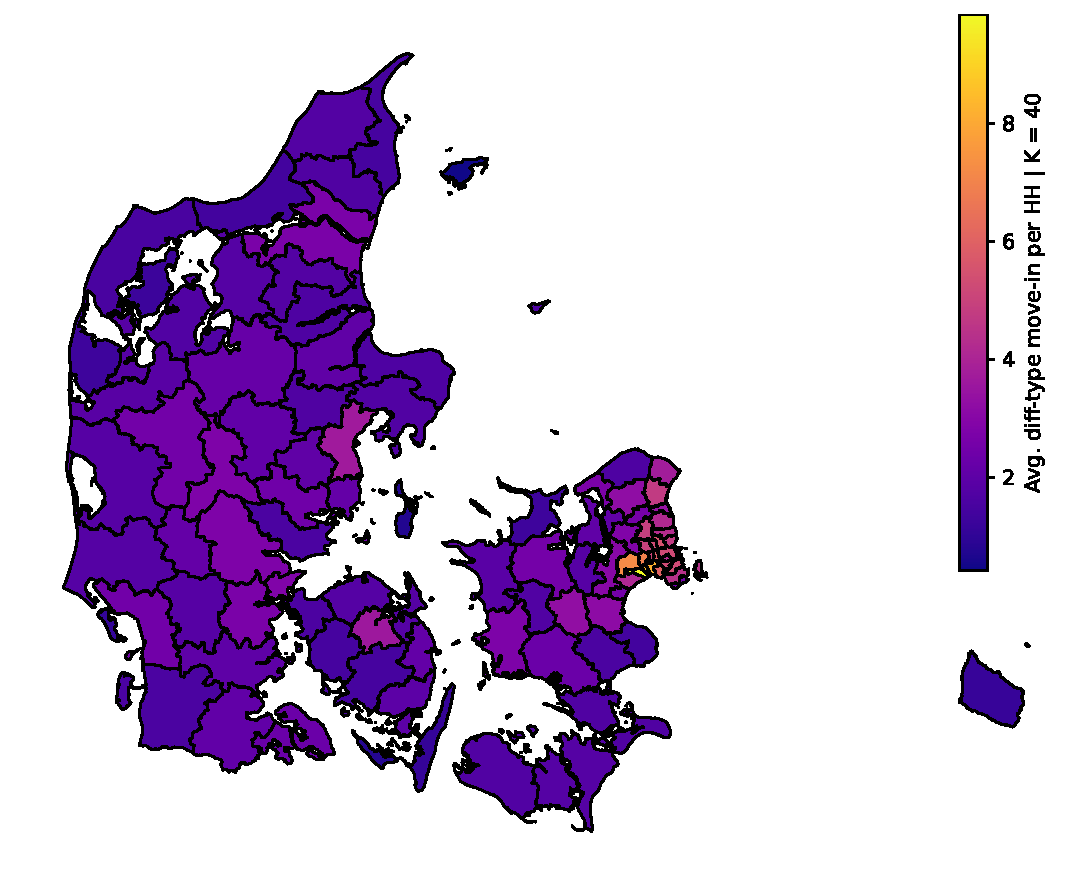
\includegraphics[width=\linewidth]{figs/dk_howdy_neighbor.pdf}
    \label{fig:incidence_different_type_dk}
\begin{tablenotes}
\item \footnotesize \textit{Note:} The figure show the variation in receiving a new-non West neighbor for native households on a national scale. Household types are split up in three types (native/non-West/West), see section \ref{sec:intro_definitions} for more details. Neighborhoods are defined in section \ref{sec:data_geospatial}.
\end{tablenotes}
\end{figure}

\begin{landscape}
\begin{figure}
\centering
\caption{Incidence of new different-type neighbors at the neighborhood level} \label{fig:health}
	\begin{subfigure}{.55\textwidth}	
	\centering
	\includegraphics[width=\textwidth]{figs/cph_howdy_neighbor_sample.pdf}	
	\caption{Copenhagen} \label{fig:incidence_different_type_cph}
	\end{subfigure}
	\begin{subfigure}{.6\textwidth}	
	\centering
	\includegraphics[width=\textwidth]{figs/greve_howdy_neighbor_sample.pdf}	
	\caption{Greve} \label{fig:incidence_different_type_greve}
	\end{subfigure}	
    
	\begin{subfigure}{.55\textwidth}	
	\centering
	\includegraphics[width=\textwidth]{figs/fredericia_howdy_neighbor_sample.pdf}	
	\caption{Fredericia} \label{fig:incidence_different_type_fredericia}
	\end{subfigure}	
\begin{tablenotes}
\item \footnotesize \textit{Note:} The figure show the variation in receiving a new-non West neighbor for native households at the \textit{neighborhood} scale for three different municipalities. Neighborhoods not in the sample are greyed out. Household types are split up in three types (native/non-West/West), see section \ref{sec:intro_definitions} for more details. Neighborhoods are defined in section \ref{sec:data_geospatial}. Municipal borders were redrawn in 2007 with "Kommunalreformen" which is what these borders represent. See Figure \ref{fig:incidence_new_non_west_neighbors_appendix} for an unconstrained version of this figure.
\end{tablenotes}
\label{fig:incidence_new_non_west_neighbors}
\end{figure}
\end{landscape}




\begin{enumerate}
    \item Map of "selected" \href{nabolagstlas.dk}{Nabolagsatlas} neighborhoods:
    \begin{itemize}
        \item Share of non-west inhabitants (1990 / 2010)
        \item Avg. no of non-west K-nearest neighbors (1990 / 2010) 
        \item Map of neighborhoods where the "experiment" occurs
    \end{itemize}
    \item Summary stats
    \begin{itemize}
        \item Dependent variable (move within 2 years of new K=3/4 nearest neighbor)
        \item Individual characteristics:
        \begin{itemize}
            \item Length of education
            \item Income (highest earner?)
            \item Age
            \item Employed
            \item ?
        \end{itemize}
        \item Neighborhood characteristics
        \begin{itemize}
            \item Median/average income,
            \item Population density
            \item Non-west share
            \item Native share
            \item No. of K=10-nearest non-west neighbors (?)
        \end{itemize}
        \item 3-4 columns (cond. on being from DK): All / new non-west neighbor (nearest) / new non-west neighbor (near)
    \end{itemize}
\end{enumerate}

\begin{landscape}
\begin{figure}
      \centering
    \caption{Temporal development of K-nearest neighbors}
    \includegraphics[width=\linewidth]{figs/temporal_knn_native_1990_2020_w_sim.pdf}
    \label{fig:incidence_different_type_dk}
\begin{tablenotes}
\item \footnotesize \textit{Note:} The figure \end{tablenotes}
\end{figure}
\end{landscape}

\subsection{Balance test}

Before diving into the main results, I perform a series of balance tests to determine any potential (mean) differences between the "control" and "treatment" group. Consider the following equation:

\begin{equation}
    X_{i, j, t} = \phi_1 \mathbb{I}[r', k=n_{nearest}] + \phi_2 \mathbb{I}[r', k = n_{near}] + \phi_3 \mathbb{I}[r', k = n_{close}] + \omega_{j, t} + \epsilon_{i, j, t} 
    \label{eq:balance_tests}
\end{equation}
Where $X$ is observables at the household and individual level Eq. (\ref{eq:balance_tests}) is exactly the same as Eq. (\ref{eq:main_eq_schelling_behavior}). 
\end{document}
